\documentclass[12pt]{article}

\usepackage[margin=1in]{geometry}
\usepackage{amsmath,amsthm,amssymb,graphicx,gensymb,multicol,mathtools}
\usepackage{hyperref}
\hypersetup{
  colorlinks=true,
  linkcolor=blue,
  filecolor=red,
  urlcolor=cyan,
}
\usepackage{color}
\usepackage[english]{babel}
\usepackage[autostyle, english = american]{csquotes}
\MakeOuterQuote{"}
\graphicspath{{figures/}}
\usepackage{tikz, pgfplots}
\pgfplotsset{compat=newest}
\allowdisplaybreaks

\usepackage{biblatex}
\addbibresource{bibfile.bib}

\newcommand{\pp}{\mathbf{p}}
\newcommand{\uu}{\mathbf{u}}
\newcommand{\vv}{\mathbf{v}}
\newcommand{\ww}{\mathbf{w}}
\newcommand{\xx}{\mathbf{\hat{x}}}
\newcommand{\yy}{\mathbf{\hat{y}}}
\newcommand{\zz}{\mathbf{\hat{z}}}
\newcommand{\rr}{\mathbf{\hat{r}}}
\newcommand{\rrr}{\mathbf{r}}
\newcommand{\ppp}{\mathbf{p}}
\newcommand{\xxx}{\mathbf{x}}
\newcommand{\nnot}{\sim \!}
\let\oldemptyset\emptyset
\let\emptyset\varnothing

%for QM:
\newcommand{\intii}{\int_{-\infty}^\infty}
\newcommand{\intoi}{\int_0^\infty}
\newcommand{\HH}{\mathbb{H}}
\newcommand{\ang}[3]{\,^{#1} {#2}_{#3}}
\usepackage{braket}
\newcommand{\tr}{\mathrm{Tr}}

%units:
\newcommand{\s}{\, \mathrm{s}}
\newcommand{\m}{\, \mathrm{m}}
\newcommand{\eV}{\, \mathrm{eV}}
\newcommand{\MeV}{\, \mathrm{MeV}}
\newcommand{\ly}{\, \mathrm{ly}}

\newenvironment{problem}[2][Problem]{\begin{trivlist}
\item[\hskip \labelsep {\bfseries #1}\hskip \labelsep {\bfseries #2.}]}{\end{trivlist}}

\begin{document}

\title{Positron Converter Model}
\author{John Mastroberti}

\maketitle

\newcommand{\dxds}{\frac{dx}{ds}}
\newcommand{\dyds}{\frac{dy}{ds}}
\newcommand{\dxdsmin}{\dxds_{\mathrm{min}}}
\newcommand{\dxdsmax}{\dxds_{\mathrm{max}}}
\newcommand{\dydsmax}{\left| \dyds \right|_{\mathrm{max}}}
\newcommand{\exes}{\texttt{converter\_simulation}}
\newcommand{\exef}{\texttt{converter\_fitter}}
\newcommand{\configfile}{\texttt{config.txt}}
\newcommand{\bmad}{\textit{Bmad}}

\tableofcontents

\newpage

\section{Introduction}

Every electron-positron collider needs a source of positrons.
At CESR, these positrons are generated in a linear accelerator using a positron converter.
Until now, we have had limited ability to optimize the design of the linac, as there was no way to model the positron converter in \bmad.
This project rectifies this problem by providing the information needed for a converter element in \bmad.
A converter element has been developed in conjunction with this project, which should enable optimizations of the linac design.


\section{Background/physics}
The positron converter provides CESR with its positrons.
The converter is a slab of heavy metal (usually tungsten), which is bombarded with electrons whose energy is on the order of $\sim 100 \MeV$.
As the incident electrons pass through the converter, they emit photons via Bremsstrahlung, which in turn decay to $e^+ e^-$ pairs:
\begin{align}
e^- + Z \rightarrow e^- + Z + \gamma \rightarrow e^- + Z + e^+ + e^-
\end{align}


\section{The converter model}
The production of positrons in the converter is a stochastic process, the details of which are computationally expensive to simulate.
It is therefore desirable to have a model for the properties of the produced positrons in terms of probability distributions.

\subsection{Coordinates}
The kinematics of a positron produced in the converter are completely described by the following quantities:
\begin{itemize}
\item
The position at which it emerges on the downstream face of the converter.

\item
Its momentum upon emerging from the converter.

\end{itemize}

With this in mind, we adopt the coordinate system shown in Figure \ref{fig:coords}.
\begin{figure}
\centering
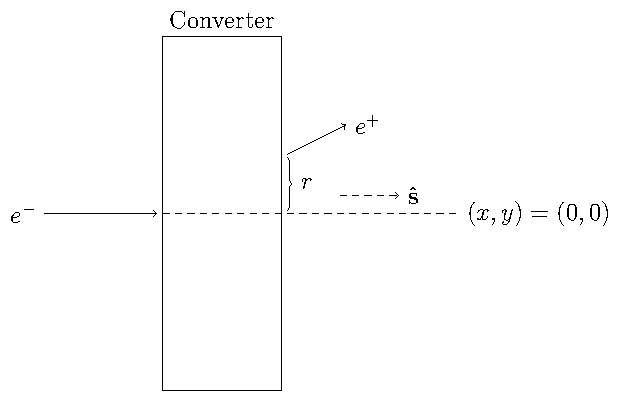
\includegraphics[width=0.6\textwidth]{coords1.pdf}
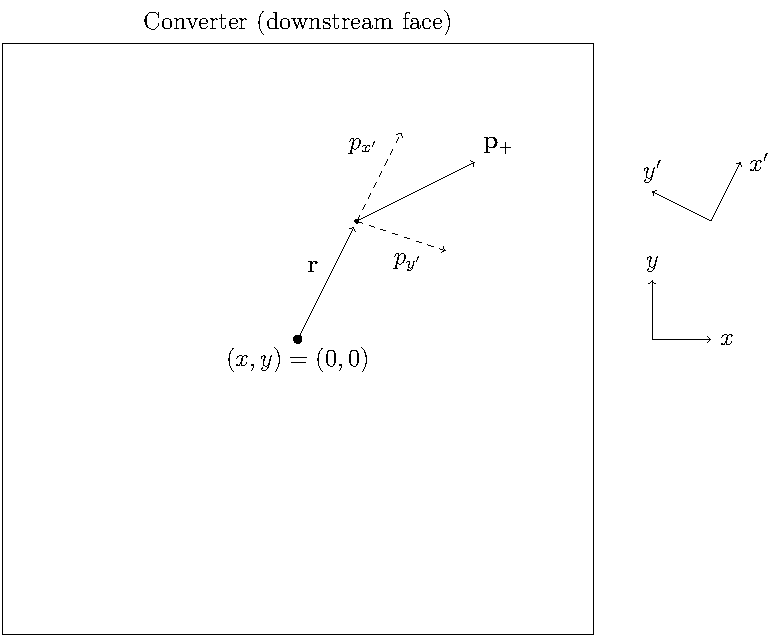
\includegraphics[width=0.8\textwidth]{coords2.pdf}
\caption{Coordinates used to describe the positrons exiting the converter.}
\label{fig:coords}
\end{figure}
We take the $z$ axis to be the direction of the incoming electron's momentum perpendicular to the surface of the converter.
The outgoing positron's position on the downstream face of the converter is then described by $r$, its distance from the $z$ axis, and the angle $\theta$ shown in the figure.
By symmetry, $\theta$ must be distributed uniformly between $0$ and $2\pi$.
We can then largely ignore this degree of freedom from our model if we define our $x$ axis in the same direction as $\rrr$.
We then choose our $y$ axis such that $(x,y,z)$ is a right handed orthogonal coordinate system.

\subsection{Probability Distributions}
With this coordinate system, the position of an outgoing positron is described entirely by $r$ (and $\theta$, chosen uniformly at random).
We choose the following three parameters to characterize the outgoing momentum:
\begin{align}
p_+ c & = \left| \mathbf{p}_+ \right| c \\
\dxds & = \frac{p_x}{p_z} \\
\dyds & = \frac{p_y}{p_z}
\end{align}
Using these four parameters to describe outgoing positrons, we seek the distribution
\begin{align}
P \left( p_+ c, r, \dxds, \dyds \right)
\end{align}
which describes the probability that an outgoing positron will attain particular values of $p_+ c$, $r$, $\dxds$, and $\dyds$.
This is not a true probability distribution, as it is not normalized to 1.
Rather, $P$ is normalized to the number of positrons produced per incoming electron:
\begin{align}
\int P \left( p_+ c, r, \dxds, \dyds \right) \, d(p_+ c) \, dr \, d \! \left( \dxds \right) d \! \left( \dyds \right) & = \frac{N_+}{N_-}
\end{align}
This normalization lets us easily account for the fact that number of positrons produced varies with the incoming electron energy and converter thickness.
To make the problem easier to work with, and to aid in visualization, we can separate $P$ into two distributions:
\begin{align}
P \left( p_+ c, r, \dxds, \dyds \right) & = P_1 \left( p_+ c, r \right) P_2 \left( \dxds, \dyds ; p_+ c , r \right),
\end{align}
where we choose $P_1$ to be normalized to $N_+/N_-$ and $P_2$ to be normalized to 1.
Note that the behavior of the converter depends on the energy of the incoming electrons and the converter's thickness, so we will have a different $P$ (and $P_1$ and $P_2$) at each incoming electron energy and target thickness.

\subsection{Obtaining $P_1$ and $P_2$}

Using Geant\cite{geant}, we simulate many incoming electrons of a given energy incident upon a converter of a given thickness.
We then record the values of $p_+ c$, $r$, $\dxds$, and $\dyds$ for each outgoing positron at the downstream face of the converter.
This data is then binned into a two-dimensional histogram by $p_+ c$ and $r$.
The sizes of the bins are chosen non-uniformly so that each bin holds approximately the same number of positrons.
This histogram is recorded and gives us a discrete sampling of $P_1(p_+c, r)$.

Then, in each $(p_+ c, r)$ bin, we fit the functional form
\begin{align}
P_2 \left( \dxds, \dyds; p_+ c, r \right) & = A \frac{1 + \beta \dxds}{1 + \alpha_x^2 \left( \dxds - c_x \right)^2 + \alpha_y^2 \left( \dyds \right)^2}. \label{eq:cauchy}
\end{align}
Since $P_2$ is normalized to $1$, $A$ is not a true fit parameter, but is fixed by normalization.
This gives us values of $c_x$, $\alpha_x$, $\alpha_y$, and $\beta$ in each $(p_+ c, r)$ bin.
The distribution of $\dxds$ and $\dyds$ is also characterized by $\dxds_{min}$, $\dxds_{max}$ and $\left| \dyds \right|_{max}$,
which define the rectangle in $\dxds \times \dyds$ space where $P_2 \left( \dxds, \dyds \right)$ is nonzero.
We then perform fits to each of the parameters $c_x, \alpha_x, \alpha_y, \beta, \dxds_{min}, \dxds_{max}, \left| \dyds_{max} \right|$ as functions of $p_+ c$ and $r$ as follows:
\begin{itemize}
\item
At each value of $p_+ c$ below a user-defined cutoff, we perform a 1D fit of the form
\begin{align}
\pi(r) = a_0 + a_1 r+ a_2 r^2 + a_3 r^3 + a_4 r^4 \label{eq:fit1}
\end{align}
for each parameter $\pi =c_x, \alpha_x, \alpha_y, \beta, \dxdsmin, \dxdsmax, \dydsmax$.
For $c_x$ and $\beta$, $a_0$ is fixed to be 0, as $c_x$ and $\beta$ must be zero at $r=0$ by symmetry.
For all other parameters, $a_4$ is fixed to be zero, so that a third degree polynomial is fit instead of a fourth degree polynomial.

\item
Above the user-defined $p_+ c$ cutoff, we perform a 2D fit of the form
\begin{align}
\pi(r) = (1 + a_1 (p_+c) + a_2 (p_+c)^2 + a_3 (p_+c)^3)
         (b_0 + b_1 r + b_2 r^2 + b_3 r^3) e^{-(k_p (p_+ c) + k_r r)} + C \label{eq:fit2}
\end{align}
for each parameter $\pi =c_x, \alpha_x, \alpha_y, \beta, \dxdsmin, \dxdsmax, \dydsmax$.
The parameter $C$ is only used for $\dxdsmax$.
Note that we set the constant term for the $p_+ c$ polynomial to $1$ in each case.
This must be done so that the fitting problem is full rank.

\end{itemize}
With these fits in hand, we have an approximation of $P_2 \left( \dxds, \dyds; p_+ c, r \right)$.



\section{Setup Instructions}
The converter modeling has two main stages.
In the first stage, the positron creation events are simulated with Geant, and the resulting positrons are binned into a histogram.
In the second stage, fits are performed for $\dxds$ and $\dyds$.
As such, we have developed two executables: one responsible for the first stage, \exes, and one responsible for the second, \exef.

\subsection{Dependencies}
\label{s:deps}
To build and run the simulation proper, \exes, you will need an up to date installation of Geant4 on your system.
See the Geant4 installation guide below for details on how to get Geant4 up and running on Linux.
You will also need \texttt{cmake} installed, although this is already a requirement for a standard \bmad \, distribution.

To build and run the fitting program, \exef, you will need the GNU Scientific Library (GSL) installed on your system.
This is distributed with \bmad, so you should already have it on your system.

Both executables require a C++ compiler with support for C++17; GCC 8 or higher should be fine.
\subsubsection{Geant4 Installation Guide}

This guide is an abbreviated version of the instructions found on \href{http://geant4-userdoc.web.cern.ch/geant4-userdoc/UsersGuides/InstallationGuide/html/}{the Geant4 website}.
\begin{enumerate}
\item
Download the source files from \url{https://geant4.web.cern.ch/support/download}.

\item
Create a directory where Geant will be installed.  I'll be using \texttt{\$HOME/geant}.

\item
\texttt{cd} to this directory and unpack the downloaded files with
\begin{verbatim}
$ tar xzvf ~/Downloads/geant4.10.06.tar.gz
\end{verbatim}
(change the version number as appropriate).

\item
Make another directory where you will build Geant with
\begin{verbatim}
$ mkdir geant4.10.06-build
\end{verbatim}

\item
\texttt{cd} to this new directory, and use \texttt{cmake} to configure the Geant4 build with
\begin{verbatim}
cmake -DGEANT4_INSTALL_DATA=ON \
      -DCMAKE_INSTALL_PREFIX=$HOME/geant/geant4.10.06-install \
      ../geant4.10.06
\end{verbatim}
The first \texttt{-D} flag will cause the necessary data sets to be downloaded when we build Geant, and the second \texttt{-D} flag sets the install directory.
If you chose a different location for installing Geant, edit this flag as needed.

Note: if you encounter the the error
\begin{verbatim}
Could NOT find EXPAT (missing: EXPAT_LIBRARY EXPAT_INCLUDE_DIR)
\end{verbatim}
at this step, try editting the file \\
\texttt{../geant4.10.06/cmake/Modules/Geant4OptionalComponentents.cmake}, \\
replacing the line
\begin{verbatim}
option(GEANT4_USE_SYSTEM_EXPAT "Use system Expat library" ON)
\end{verbatim}
with
\begin{verbatim}
option(GEANT4_USE_SYSTEM_EXPAT "Use system Expat library" OFF)
\end{verbatim}
and then re-run the above \texttt{cmake} command.

\item
After \texttt{cmake} finished running, start building Geant with
\begin{verbatim}
$ make -jN
\end{verbatim}
where \texttt{N} is the number of threads you want to use for the compilation.

\item
Once the compilation has finished, install to the install directory you specified in step 5 with
\begin{verbatim}
$ make install
\end{verbatim}

\item
The file \texttt{\$HOME/geant/geant4.10.06-build/geant4make.sh} must be sourced to add Geant4 to your path.
To do so, add the following to your \texttt{.bashrc}:
\begin{verbatim}
cd $HOME/geant/geant4.10.06-build && source geant4make.sh && cd -
\end{verbatim}
Again, if you chose a different location for installing Geant, modify this as necessary.

\end{enumerate}



\subsection{Compiling the Executables}
The converter simulation and fitting programs are distributed as part of the \texttt{util\_programs} project, which is included in a standard \bmad \, distribution.
If you are working with a release instead of a distribution, you can pull down the latest version of the \texttt{util\_programs} project with
\begin{verbatim}
$ svn co https://accserv.lepp.cornell.edu/svn/trunk/src/util_programs
\end{verbatim}
Once you have \texttt{util\_programs} on your system, you will need to add
\begin{verbatim}
export ACC_BUILD_TEST_EXES="Y"
\end{verbatim}
to your \texttt{.bashrc}, and then start a new shell.
\texttt{cd} to the \texttt{util\_programs} folder, and then simply run \texttt{mk} to build \exes \, and \exef \, (or \texttt{mkd} for debug builds).



\section{How to run the programs}

\subsection{Configuration}
Both \exes \, and \exef \, are configured by editing the file \configfile, which should be in the working directory where you run both executables.
Each line in this file should have the form
\begin{verbatim}
setting = value
\end{verbatim}
Comments can be inserted with an exclamation mark \texttt{!} and last until the end of the line.
An example config file, with all available settings listed, is shown below.
\begin{verbatim}
! Example configuration file
! The ! introduces a comment that lasts until the end of the line
target_material = tungsten ! Defines the converter material
target_thickness = 6.35 mm, 1.0 cm ! Defines the target thicknesses to be simulated
pc_in = 300 MeV, 500 MeV, 1 GeV ! Defines the electron energies to be simulated
out_pc_min = 0 ! Minimum pc cutoff for outgoing positrons, defaults to 0
out_pc_max = 100000000 ! Maximum pc cutoff for outgoing positrons (in eV here)
dxy_ds_max = 10 ! Maximum cutoff for the magnitude of dx/ds
                ! and dy/ds allowed for outgoing positrons
output_directory = sim_data ! Name of the directory where data will be output,
                            ! should be specified relative to the working directory
                            ! Defaults to sim_data
num_bins = 15 ! Number of bins to use for both pc and r histogram binning
              ! with just this line, you would have a 15x15 histogram
              ! Defaults to 15
num_pc_bins = 12 ! Number of pc bins to use for histogram binning
num_r_bins = 20 ! Number of r bins to use for histogram binning
fit_crossover = 10 MeV ! For alpha and beta fits, this defines the
                       ! point where the fitter transitions from 1D
                       ! to 2D fits, defaults to 10 MeV
\end{verbatim}
\newcommand{\targetm}{\texttt{target\_material}}
\newcommand{\targett}{\texttt{target\_thickness}}
\newcommand{\pcin}{\texttt{pc\_in}}
\newcommand{\outpcmin}{\texttt{out\_pc\_min}}
\newcommand{\outpcmax}{\texttt{out\_pc\_max}}
\newcommand{\dxydsmax}{\texttt{dxy\_ds\_max}}
\newcommand{\outdir}{\texttt{output\_directory}}
\newcommand{\numbins}{\texttt{num\_bins}}
\newcommand{\numrbins}{\texttt{num\_r\_bins}}
\newcommand{\numpcbins}{\texttt{num\_pc\_bins}}
\newcommand{\fitxpt}{\texttt{fit\_crossover}}

All settings accept a single value, except for \pcin \, and \targett, which accept a comma separated list of values.
The settings \outpcmin, \outdir, \numbins, and \fitxpt \, have default values, while the settings \targetm, \targett, \pcin, \outpcmax, and \dxydsmax \, must be specified in the file.

The settings \pcin, \outpcmin, and \outpcmax \, take values with dimensions of energy.
These default to eV if no unit is specified, although \texttt{MeV} and \texttt{GeV} can be added as suffixes to use MeV and GeV instead as shown in the sample file.
The \targett \, setting takes values with dimensions of length.
The default unit is meters, although \texttt{cm} and \texttt{mm} are supported as well.

The settings \numbins, \numpcbins, and \numrbins \, control the number of bins used in the histogram.
If you only provide a value for \numbins, it will be used for both the number of $p_+c$ bins and then number of $r$ bins.
If you provide \numpcbins \, or \numrbins \, in your config file, this value will supersede \numbins \, for the number of $p_+ c$ or $r$ bins respectively.
If you do not set \numbins \, in your config file, you must set both \numpcbins \, and \numrbins.

\subsection{The Simulation Program}

To run \exes \, and perform the converter simulation, first create and edit the configuration file \configfile, and place it in your working directory.
Then, just run
\begin{verbatim}
$ converter_simulation
\end{verbatim}
at your command prompt.
The program will parse your config file and report the settings it read, and report if there are any problems reading your config file.
It will then verify that the directory you set for \outdir \, does not exist or is empty, and will ask you if you want to overwrite it if it already exists.
Then, for each value of \pcin \, and \targett \, specified in the config file, the program will simulate many positron events for those settings.
For example, with the above config file, six simulations will be run with the following settings:
\begin{itemize}
\item
300 MeV \pcin \, and 6.35 mm \targett

\item
500 MeV \pcin \, and 6.35 mm \targett

\item
1 GeV \pcin \, and 6.35 mm \targett

\item
300 MeV \pcin \, and 1 cm \targett

\item
500 MeV \pcin \, and 1 cm \targett

\item
1 GeV \pcin \, and 1 cm \targett
\end{itemize}

Depending on your computer and the number of different simulations that need to be run, this step may take several hours.
%Fortunately, this only has to be done once to set up the \bmad \, converter element.


\subsection{The Fitting Program}

Once the simulations are complete, just run
\begin{verbatim}
$ converter_fitter
\end{verbatim}
in the same directory where you ran \exes.
\exef will re-parse your config file for the settings it needs, and will again report on any errors it encounters.
It then performs the fit from Equation \ref{eq:cauchy} in each of the $(p_+c, r)$ bins for each simulation.
At this stage, the program may report that the fitting iteration limit has been reached a few times; this is not cause for concern.
Once this step is complete, and the program has obtained values of $c_x$, $\alpha_x$, $\alpha_y$, and $\beta$ in each $(p_+c, r)$ bin,
it performs the fits from Equations \ref{eq:fit1}-\ref{eq:fit2} on these fit parameters.
Finally, the results of the simulation, as well as the results of the fits, are output to the file \texttt{converter.bmad}, located in the \outdir \, specified in the config file.

\section{Output from the Programs}

\subsection{Simulation Output}

After running the \exes \, program, the directory specified by the \texttt{output\_directory} setting in the configuration file will exist in your working directory.
Inside it, there will be one file of the format '\texttt{E\{pc\_in\}\_T\{thickness\}\_er.dat}', for each incoming $p_- c$ and target thickness specified in the configuration file, where \texttt{pc\_in} and \texttt{thickness} are the $p_- c$ and thickness in MeV and cm respectively.
These files contained the binned data which approximate $P_1(p_+ c, r)$.
The output directory will also contain a directory \texttt{dir\_dat}, with subdirectories \texttt{E\{pc\_in\}\_T\{thickness\}\_er.dat} for each $p_- c$ and target thickness combination.
Each of these directories will contain files named \texttt{E\{pc\_out\}\_r\{r\_out\}\_bin.dat}, which contain the binned $\dxds$ and $\dyds$ data used by \exef.

\subsection{Fitting Output}

After running the \exef \, program, the output directory will also contain a file called \texttt{converter.bmad}.
This file aggregates all the information about $P_1$ and $P_2$ at each $p_+ c$ and target thickness tested, and is designed for use with a \bmad \, converter element.

\subsubsection{Gnuplot Files}

\exef \, also generates several gnuplot scripts for inspecting the quality of the obtained fits.
These are all written to the individual \texttt{E\{\}\_r\{\}} directories under \texttt{dir\_dat}.

Each of the $(p_+ c, r)$ bins gets two gnuplot scripts: \texttt{cauchy\_E\{pc\_out\}\_r\{r\_out\}.gp} and \texttt{meta\_E\{pc\_out\}\_r\{r\_out\}.gp}.
The scripts with the \texttt{cauchy} prefix display the distribution $P_2$ obtained by directly fitting Equation \ref{eq:cauchy} to the data in each bin.
The scripts with the \texttt{meta} prefix display the distribution $P_2$ obtained from evaluating the fits from Equations \ref{eq:fit1}-\ref{eq:fit2} to the Cauchy fit parameters.

\exef \, also outputs scripts for viewing the fits from Equations \ref{eq:fit1}-\ref{eq:fit2} across all $(p_+ c, r)$ bins.
These are named \texttt{c\_x\_master.gp},
\texttt{a\_x\_master.gp},
\texttt{a\_y\_master.gp},
\texttt{beta\_master.gp},
\texttt{dxds\_min\_master.gp},
\texttt{dxds\_max\_master.gp},
and \texttt{dyds\_max\_master.gp}.

To view any of these plots, simply open Gnuplot in the \texttt{E\{\}\_T\{\}} directory of interest, and call the script.
For example:
\begin{verbatim}
$ pwd
/home/user/sim_data/dir_dat/E300_T0.635
$ gnuplot

        G N U P L O T
        Version 5.2 patchlevel 8    last modified 2019-12-01

        Copyright (C) 1986-1993, 1998, 2004, 2007-2019
        Thomas Williams, Colin Kelley and many others

        gnuplot home:     http://www.gnuplot.info
        faq, bugs, etc:   type "help FAQ"
        immediate help:   type "help"  (plot window: hit 'h')

Terminal type is now 'qt'
gnuplot> call 'c_x_master.gp'
\end{verbatim}
This will open the plot for $c_x$ across all $(p_+ c, r)$ bins for $p_+ c = 300$ MeV, $T = 0.635$ cm.

\appendix

\section{Notes for ACC Computer Users}

As detailed in Section \ref{s:deps}, building \exes and \exef requires GSL, Geant, and a C++ compiler with support for C++17.
GSL is already available on the lab machines, and a build of Geant is provided at \texttt{/nfs/acc/temp/jmm699/geant}.
To get access to this Geant build, you can simply add the following to your \texttt{.bashrc}:
\begin{verbatim}
cd /nfs/acc/temp/jmm699/geant/geant4.10.06.p01-build && source geant4make.sh && cd -
\end{verbatim}
As for the C++ compiler, you can get access to GCC 8.3 by adding
\begin{verbatim}
source /opt/rh/devtoolset-8/enable
\end{verbatim}
to your \texttt{.bashrc}.








\printbibliography


\end{document}
